\documentclass[12pt]{article}

\usepackage{amsmath,amssymb,amsfonts,amsbsy}
%\usepackage{cite}
\usepackage{graphicx}
\usepackage[margin=20mm]{geometry}
\usepackage{wrapfig}
\usepackage[pagewise,displaymath]{lineno}
\usepackage{subfig}
\usepackage{epsfig}
\usepackage{authblk}
\usepackage[d]{esvect}
\usepackage{calc}
\usepackage[colorlinks=false,bookmarks=false,pageanchor=true]{hyperref}

\newcommand{\missET}{\vv{\not{\!\!E}}_T}
\newcommand{\abs}[1]{\lvert#1\rvert}

\begin{document}

\setcounter{section}{0}
\setcounter{subsection}{0}
\setcounter{equation}{0}
\setcounter{figure}{0}
\setcounter{footnote}{0}
\setcounter{table}{0}


\title{Measurement of Vector Boson Asymmetry in Transveresely Polarized $pp$
Collisions at RHIC}

\author{Salvatore Fazio\thanks{fazio@bnl.gov}}
\author{Dmitri Smirnov\thanks{dsmirnov@bnl.gov}}

\affil{Physics Department, Brookhaven National Lab}
\date{\today}

\maketitle

\newpage
\tableofcontents 

\newpage
\linenumbers


\section{Introduction}
%{{{

This study is the first attempt to measure the single spin asymmetry for weak bosons produced
in transversely polarized proton collisions at STAR. 

Transversely polarized spin effects have been an extremely active topic among experiment and theory in the past years, because of their connection to transverse momentum dependent (TMD) distributions (leading to a multi-dimensional picture of the proton) and a possible test of the framework and the underlying theory of perturbative QCD. For a quantitative application of the TMD framework to transverse single-spin asymmetries measured in proton-proton collisions, the required two scales (typically $Q^{2}$ and $p_{T}$) are not well defined, excepted for Drell-Yan di-lepton (DY) and $W^{\pm}$,$Z^{0}$ boson production. DY production has been at the center of attention for the non-universality test of the so-called Sivers TMD function, %it requires large integrated luminosities and efficient background reduction. The high mass of $W$-bosons naturally provides a hard $Q^{2}$ scale already and their transverse asymmetries can be directly applied to a global TMD analysis.
$f^{\perp}_{1T}$, which describes the correlation of parton transverse momentum with the transverse spin of the nucleon.  There is evidence of a quark Sivers effect in semi-inclusive DIS (SIDIS) measurements where the quark Sivers function is associated with a final state effect from the gluon exchange between the struck quark and the target nucleon remnants. On the other hand, for the virtual photon production in the Drell-Yan process, the Sivers asymmetry appears in the initial state of the interaction. As a consequence, the quark Sivers functions are of opposite sign in SIDIS and in Drell-Yan
%
\begin{equation}
f^\text{SIDIS}_{q/h^\uparrow} (x, k_\perp) = - f^\text{DY}_{q/h^\uparrow} (x, k_\perp).
\end{equation}

The experimental test of this sign change is one of the open questions in hadronic physics, and can provide insights on the TMD factorization. While luminosities required for a meaningful measurement of asymmetries in Drell-Yan production are challenging, $W^{\pm}$ and $Z^{0}$ bosons production is equally sensitive to the predicted sign change and can be well measured at the STAR experiment.  The results can also provide essential input to study the new theoretical concept of evolution effects of transverse momentum dependent distribution functions, because of the high $Q^{2}$ in the $W\rightarrow e \nu$ production due to the large boson mass. The STAR experiment at RHIC is currently the only place in the world where these effects can be tested.

The transverse single spin asymmetry, $A_N$, has been derived in~\cite{Kang:2009bp} and its parametrization is based on the fits to SIDIS data.
Predictions show that a transverse asymmetry solely calculated from the lepton decay is diluted~\cite{Kang:2009bp} if compared to the same asymmetry calculated directely from the produced boson. 
Thus, a full reconstruction of the produced boson kinematics is crucial for a meaningful measurement.
The present analysis is based on a data sample collected in the year 2011 at STAR using transversely polarized proton-proton collisions at the center-of-mass energy of $\sqrt(s)=500~GeV$, the total integrated luminosity is $L_{int} = 25$ pb$^{-1}$. In the present woek we use this exploratory run to test the possibility of fully reconstructing the $W^{\pm}$ boson kinematics at STAR, using the lepton decay and all other particles in the recoil from the initial hard scattering. This analysis also includes a first look at $A_{N}$ in $Z^{0}$ production. 
%A proposed measurement with increased statistics in 2016 will be directly competitive with a Drell-Yan measurement in pion-proton scattering at CERN.

%The single spin asymmetry (SSA) $A_N$ for the $W$ bosons and the lepton $l$
%from the $W$ decay has been derived in \cite{Kang:2009bp}. It is
%parametrized based on the fits of SIDIS data and given as a function of
%direction and transverse momentum. For the case of $W$ we have:
%
%\begin{equation}
%A^W_N = A^W_N(y_W, \phi_W, q_T) \equiv A_N(y, \phi, p_T) = A_N(\Omega, p_T),
%\label{eq:asym_wboson}
%\end{equation}
%
%where $\Omega = \{y, \phi\}$ is simply used as a shorthand for the direction of
%the particle in the lab frame. Similarly, for the lepton the expectated
%asymmetry depends on the direction of the lepton and its transverse momentum:
%
%\begin{equation}
%A^l_N = A^l_N(\eta_l, \phi_l, p_T) \equiv A_N(y, \phi, p_T) = A_N(\Omega, p_T)
%\label{eq:asym_lepton}
%\end{equation}

%}}}


\section{The $W^{\pm}$ selection and asymmetry measurement}
A data sample characterized by the $W$ signature has been selected, mostly requiring an isolated high $P_{T} > 25$~GeV electron and a total recoil $P_{T} >18$~GeV.
In order to fully reconstruct the $W$ kinematics the momenta of all $W$ decay
products must be measured. The momentum of the neutrino produced in the leptonically decayed $W$
cannot be measured and can only be indirectly deduced from conservation of the total momentum. 
in the $W$ events produced at $\sqrt{s}=500$~GeV
at STAR we can assume that most of the missing energy, $\missET$ is carried by the neutrino from the
$W$ decay. The assumption ${P}_{\nu, T} \approx \missET$ is based on the
fact that only very little energy is left for anything other than $W$ production
from the primary hard scattering.
In the transverse plane the initial momentum of the system of interacting partons is negligible
and so must be the vector sum of all final particles momenta. We define the
missing transverse energy as a vector restoring the balance in the event:

\begin{equation}
\missET = - \sum_{i \in \parbox[t]{\widthof{\tiny clusters}}{\tiny tracks, clusters}} \vv P_{i,T}.
%miss ET = - \sum_{clusters}{jets, tracks, clusters} P_{i,T}.
\end{equation}

In a typical collider detector like STAR the problem with measuring the missing momentum from the hadronic recoil
is that particles with very high rapidities escape the detector. At the same time, the beam remnants with high
longitudinal momentum carry away only a little portion of the total transverse
momentum. We accounted for the non measured tracks and clusters by using an event-by-event Monte Carlo 
correction to the data.
Knowing its transverse momentum, the longitudinal component of the neutrino's momentum can be reconstructed solving the quadratic equation for the invariant mass of the produced boson

\begin{equation}
\label{eq_InvMass}
M^{2}_{W}=(E_{e}+E_{\nu})^{2} - (\vv P_{e}+\vv P_{\nu})^{2},
\end{equation}
where we assumed the nominal value of the $W$-mass.  Eq.~\ref{eq_InvMass} leads to two possible solutions for $P_{L}^{\nu}$, we chose the smaller one in magnitude because it leads to a much smaller fraction of mis-reconstructed events in our kinematic domain.

Background sources coming from $W^{\pm}\rightarrow \tau^{\pm} \nu_{\tau}$, $Z^{0} \rightarrow e^{+}e^{-}$ and QCD events have been estimated to be contained within maximum a few percent of the selected sample.

%For the $A_{N}$ measurement we are interested in the interaction
%$p^{\uparrow/\downarrow} p \to W^\pm \to e^\pm \nu_e$ in which the spin direction of one
%of the protons is irrelevant, \textit{i.e} unpolarized protons. 
In measuring $A_{N}$ we assume that the beam polarization vector does not significantly
deviate from the vertical direction given by the normal unit vector $\vec n$
along the vertical $y$ axis, $P \equiv \vec{P} \cdot \vec{n}$. 
We also assume the same magnitude of the polarization vector for
spin-up and spin-down bunches, \textit{i.e.} $P = P_\uparrow = P_\downarrow$.
%For unpolarized cross section $\sigma_0 \equiv (\sigma_\uparrow + \sigma_\downarrow)/2$ 
The single spin asymmetry $A_N$ is expressed as:

\begin{align}
\label{eq_anapower}
A_N &= \frac{\sigma_\uparrow - \sigma_\downarrow}{\sigma_\uparrow +
   \sigma_\downarrow}.
\end{align}

We bin our data sample in three observable variables, $\{y, \phi, P_T\}$, of the produced boson. Thus, 
we calculated $A_{N}$ using the square root formula~\cite{sqrtFormula}, which helps to cancel out unwanted effects due to geometry and luminosity.

\begin{align}
A_{N } sin(\phi)= \frac{1}{<P>}
\frac{\sqrt{N_\uparrow(\phi_i)N_\downarrow(\phi_i+\pi)} - \sqrt{N_\uparrow(\phi_i+\pi)N_\downarrow(\phi_i)} } 
{\sqrt{N_\uparrow(\phi_i)N_\downarrow(\phi_i+\pi)} + \sqrt{N_\uparrow(\phi_i+\pi)N_\downarrow(\phi_i)}},
\end{align}
where $N$ is the number of recorded events in the $i-th$ bin with a certain spin ($\uparrow \downarrow$) configuration in the ``left'' ($\phi_{i}$) or in the ``right'' ($\phi_{i} + \pi$) side of the detector and $<P>\simeq 53\%$ is the average RHIC beam polarization for 2011 transverse p+p run.  
For the asymmetry measurement the polarization of one of the beams is ignored by combining the
yields with opposite spins, \textit{e.g.}

\begin{align}
N_{\uparrow}   \equiv N_{\uparrow0}   &= N_{\uparrow\uparrow}   + R_{\frac{0\uparrow}{0\downarrow}} N_{\uparrow\downarrow},\\
N_{\downarrow} \equiv N_{\downarrow0} &= N_{\downarrow\uparrow} + R_{\frac{0\uparrow}{0\downarrow}} N_{\downarrow\downarrow},
\end{align}

\noindent
where re-weighting factor $R_{\frac{0\uparrow}{0\downarrow}}$ addresses a
possible relative difference in the spin-up and spin-down intensities of the
other beam. Studies have shown that $R_{\frac{0\uparrow}{0\downarrow}} \approx
1$ with good precision.


\section{Background estimation}

The background sources considered in this analysis are: 
$Z^{0} \rightarrow e^+e^-$; 
$W^{\pm} \rightarrow \tau\nu \rightarrow e^+e^-\nu$; 
QCD events decaying into leptons, 
where one of the final leptons is not detected.
The first two sources have been evaluated using PYTHIA sample simulates with.... STAR Geometry... and embedded to 2011 transverse zero-bias events.


\section{Correction for Background}
%{{{

In this analysis an optimal set of cuts is applied to select signal enriched
events without significant loss in the final statistics. The final yields
include some fraction of background events $f_B$ which along with the signal
asymmetry contribute to the measured asymmetry $A_N$. In order to extract the
signal asymmetry we decompose $A_N$ as following:
%
\begin{equation}
A_N = f_\text{sig} A^\text{sig}_N + f_B A^B_N,
\label{eq:asym_bkg}
\end{equation}
%
with $f_\text{sig} = 1 - f_B$. The last term in \eqref{eq:asym_bkg} may include
contributions from various backgrounds which will be discussed later. The
background fractions and asymmetries have to be estimated in order to extract
the final asymmetry of the signal:
%
\begin{equation}
A^\text{sig}_N = \frac{A_N + f_B A^B_N}{1 - f_B}
\label{eq_bkg_corr}
\end{equation}

%}}}


\section{Sivers Sign Change Extraction}
%{{{

A binned likelihood method can be used to check the sensitivity of our data to
the sign of the Sivers function. A direct way of doing this is to compare the
measured asymmetry \eqref{eq:asym_sqrt} with background corrected expectations
from \eqref{eq:asym_bkg}. The signal asymmetry $A^\text{sig}_N$ in this case
directly comes from the model predictions~\eqref{eq:asym_wboson} or
\eqref{eq:asym_lepton}. The simplest likelihood function can be constructed as a
product of gaussian terms over all bins:
%
\begin{equation}
L = \prod\limits_i G(A_{N,i}, \sigma_{A_{N,i}}; A^\text{sig}_{N,i}).
\end{equation}
%
Alternatively, the Sivers sign can be extracted from the Poisson probabilities
of measured given the expected yields.
%
\begin{equation}
L = \prod\limits_{i,\uparrow,\downarrow} P(N_i; N^\text{sig}_{i} + B_i).
\end{equation}
%
While this method is more ``classic'' it requires the explicit knowledge of
luminosity, unpolarized cross section, and efficiencies. These values are
needed to calculate the expected number of events using \eqref{eq:yield}. The
two methods are expected to give consistent results. However, the difference
can be more perceptible when systematic effects are taken into account.

%}}}


\section{Reconstruction of $W$ Kinematics}
%{{{

In order to fully reconstruct the $W$ kinematics the momenta of all $W$ decay
products must be measured. The neutrino produced in the leptonically decayed $W$
cannot be measured in our detector. The momentum of the neutrino can only be
indirectly deduced from conservation of the total momentum. In the transverse
plane the initial momentum of the system of interacting partons is negligible
and so must be the vector sum of all final particles momenta. We define the
missing transverse energy as a vector restoring the balance in the event:

\begin{equation}
\missET = - \sum_{i \in \parbox[t]{\widthof{\tiny clusters}}{\tiny jets, tracks, clusters}} \vv P_{i,T}.
\end{equation}

In a typical collider detector like STAR the problem with measuring the
longitudinal component of the missing energy is that the total particle momentum
along the beam direction is not measured due to particles with very high
rapidities escape the detector. However, in the $W$ events produced at 250~GeV
at STAR we can assume that most of the $\missET$ is due to the neutrino from the
$W$ decay. The assumption $\vec{p}_{\nu, T} \approx \missET$ is based on the
fact that only very little energy is left for anything other than $W$ production
from the primary hard scattering. At the same time, the beam remnants with high
longitudinal momentum carry away only a little portion of the total transverse
momentum. With an assumption that the boson is produced with mass $M_W$ we can
reconstruct the $z$ component of the neutrino's momentum. For the invariant mass
we have:

\begin{align}
M^2_W &= (E_l + E_\nu)^2 - (\vec{p}_l + \vec{p}_\nu)^2,\\
M^2_W/2 &= \abs{\vec{p}_l} \abs{\vec{p}_\nu} - \vec{p}_{l,T} \cdot \vec{p}_{\nu,T} - \vec{p}_{l,z} \cdot \vec{p}_{\nu,z},
\end{align}

\noindent
where we neglected the masses of the both neutino and lepton. Introducing a
shorthand expression for $A = M^2_W/2 + \vec{p}_{l,T} \cdot \vec{p}_{\nu,T}$,
after trivial arithmetics we arrive to a quadratic equation for $p_{\nu,z}$:

\begin{align}
\abs{\vec{p}_{l,T}}^2 p^2_{\nu,z} - 2A p_{l,z} p_{\nu,z} + \abs{\vec{p}_{\nu,T}}^2 \abs{\vec{p}_{l}}^2 - A^2 = 0.
\end{align}

This equation has two solutions:

\begin{align}
p_{\nu,z} = \frac{ A p_{l,z} \pm \sqrt{ A^2 p^2_{l,z} - \abs{\vec{p}_{l,T}}^2 (\abs{\vec{p}_{\nu,T}}^2 \abs{\vec{p}_{l}}^2 - A^2) } }{\abs{\vec{p}_{l,T}}^2}
\end{align}

%}}}


\section{Preliminary Sensitivity Studies}
%{{{

In 2011 transversely polarized proton-proton beams were brought into collisions
at STAR with a center of mass energy of $500~GeV$. In this regime the $W$ is
expected to have a relatively small $P_T \sim 2$~GeV as confirmed by a
Monte-Carlo simulation in Figure~\ref{fig:MC_W_Pt}. We use PYTHIA~6.8 to
simulate $W^\pm \to e^\pm \nu_e$ to the LO with unpolarized beams. Expected
kinematic distributions of the lepton coming from the $W$ decay is shown in
Figure~\ref{fig:MC_W_eta}.

\begin{figure}[tbh]
\begin{center}
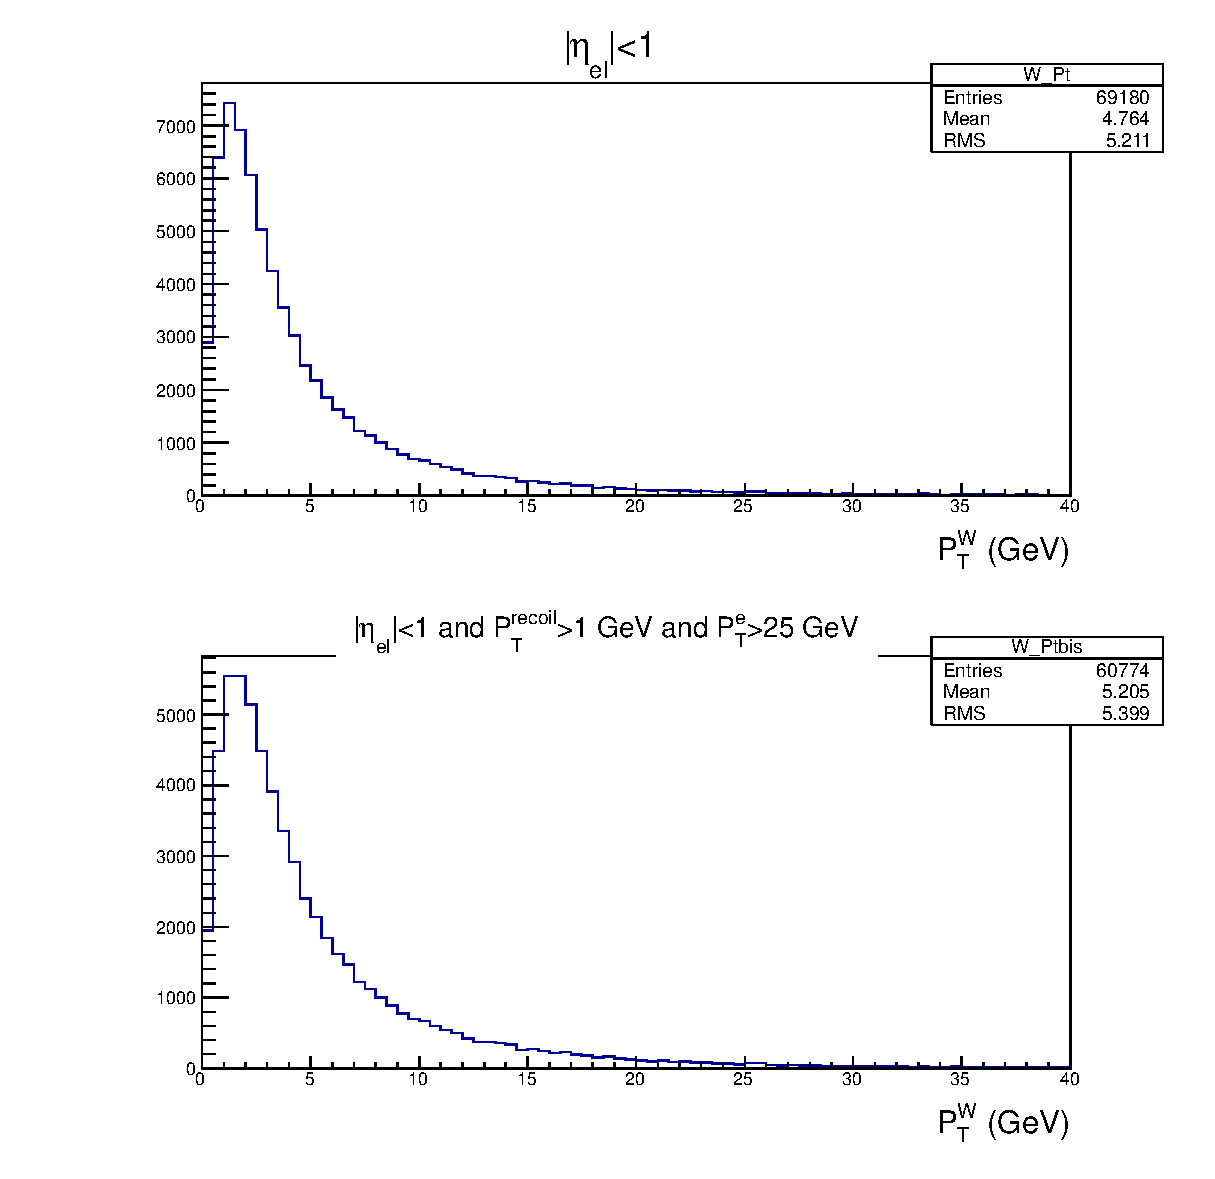
\includegraphics[width=10cm]{images/W_Pt}
\end{center}
\caption{Expected distribution of the transverse momentum of the produced W boson, $P^W_T$.}
\label{fig:MC_W_Pt} 
\end{figure}

\begin{figure}[tbh]
\begin{center}
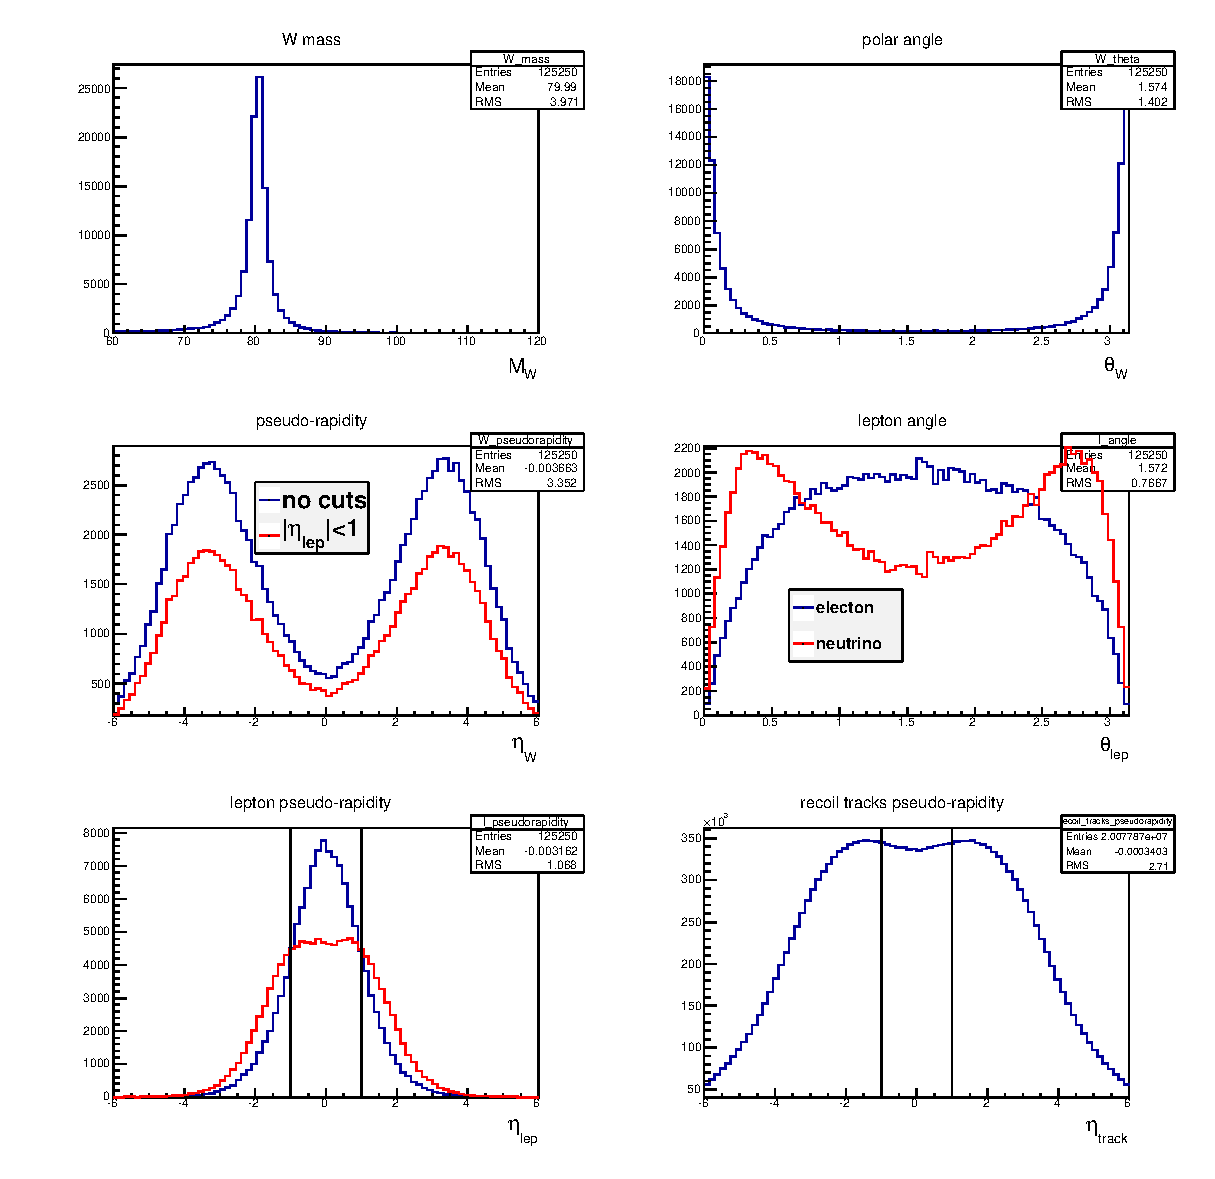
\includegraphics[width=14cm]{images/W_rapidity}
\end{center}
\caption{W-mass; polar angles and pseudo rapidity distributions of the produced W, the decay leptons and the recoil tracks.}
\label{fig:MC_W_eta} 
\end{figure}

Most of the recoil tracks in the BARREL region are expected to carry a very
small fraction of the energy as shown in fig.~\ref{fig:MC_recoil_Efrac}.

\begin{figure}
\centering
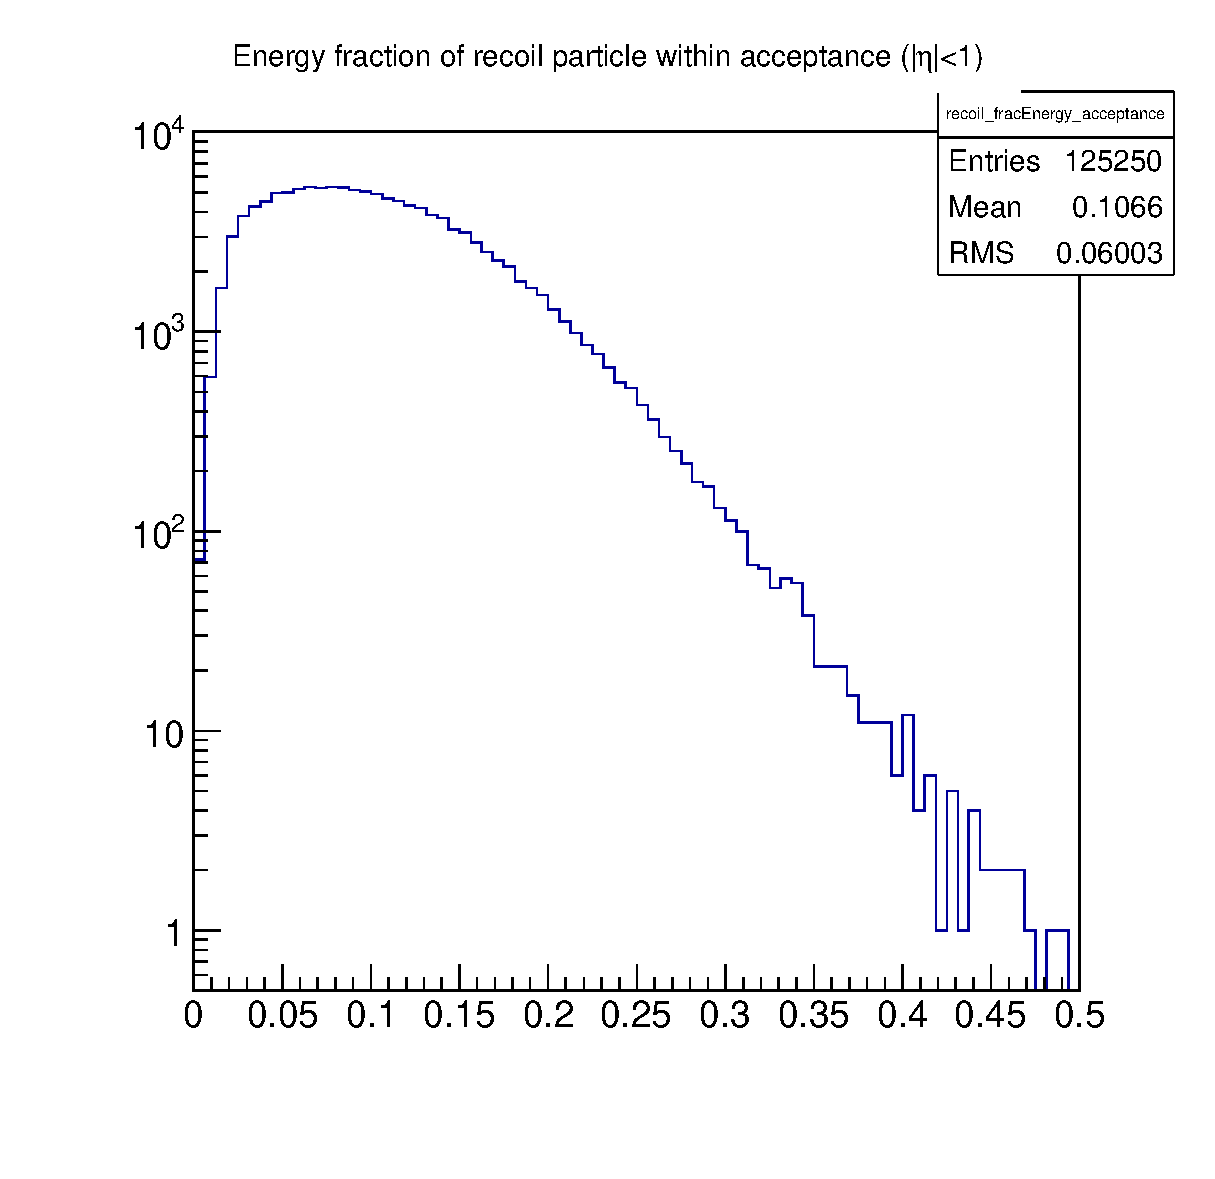
\includegraphics[height=0.5\textheight]{images/recoil_energy_frac.eps}
\caption{Expected fraction of energy carried by recoil particles within the BARREL region ($|\eta|<1$).}
\label{fig:MC_recoil_Efrac} 
\end{figure}

We can use MC to correct for the missing $P_{T}$ in the recoil tracks due to
the limited acceptance of the STAR detector. \textit{Such a procedure will
introduce a model-dependent systematic which will grow with the value of the
correction.}
%Nevertheless values of the corrections up to 30-40\% are considered acceptable...

We estimate the statistical power of the $A_N$ measurement for an integrated
luminosity of $300~\text{pb}^{-1}$. As a basis we use the total $W^\pm$ and
$Z^0$ yields observed at STAR in Run 9. The $W$ and $Z$ candidate events,
$N_\text{obs}$, along with the backgound numbers, $N_\text{bkg}$, are borrowed
from the earlier STAR analysis~\cite{WCrossSecRun9} that reported the production
cross section using $\approx 13~\text{pb}^{-1}$ of inegrated luminosity:
%
%$N_{W/Z} = N_\text{obs} - N_\text{bkg}$

\begin{align*}
N_{W^+} &= 496 - 37 = 459,\\
N_{W^-} &= 148 - 26 = 125,\\
N_Z &= 13 - 0 = 13.
\end{align*}

To reflect the expected increase in the integrated luminosity we scale the
above numbers a factor $\approx 23$. In order to illustrate the sensitivity of
the future measurement to the non-vanishing $W$ and $Z$ $A_N$ we calculate the
relative yields in bins of the boson rapidity from the MC sample. The expected
statistical power of $A_N$ in bins of $W$ rapidity is shown in
Figure~\ref{fig:MC_Wmeas_stat} for $W^+$ and $W^-$ respectively compared with
theoretical prediction from~\cite{Kang:2009bp}.

\begin{figure}
\subfloat[$W^+$]{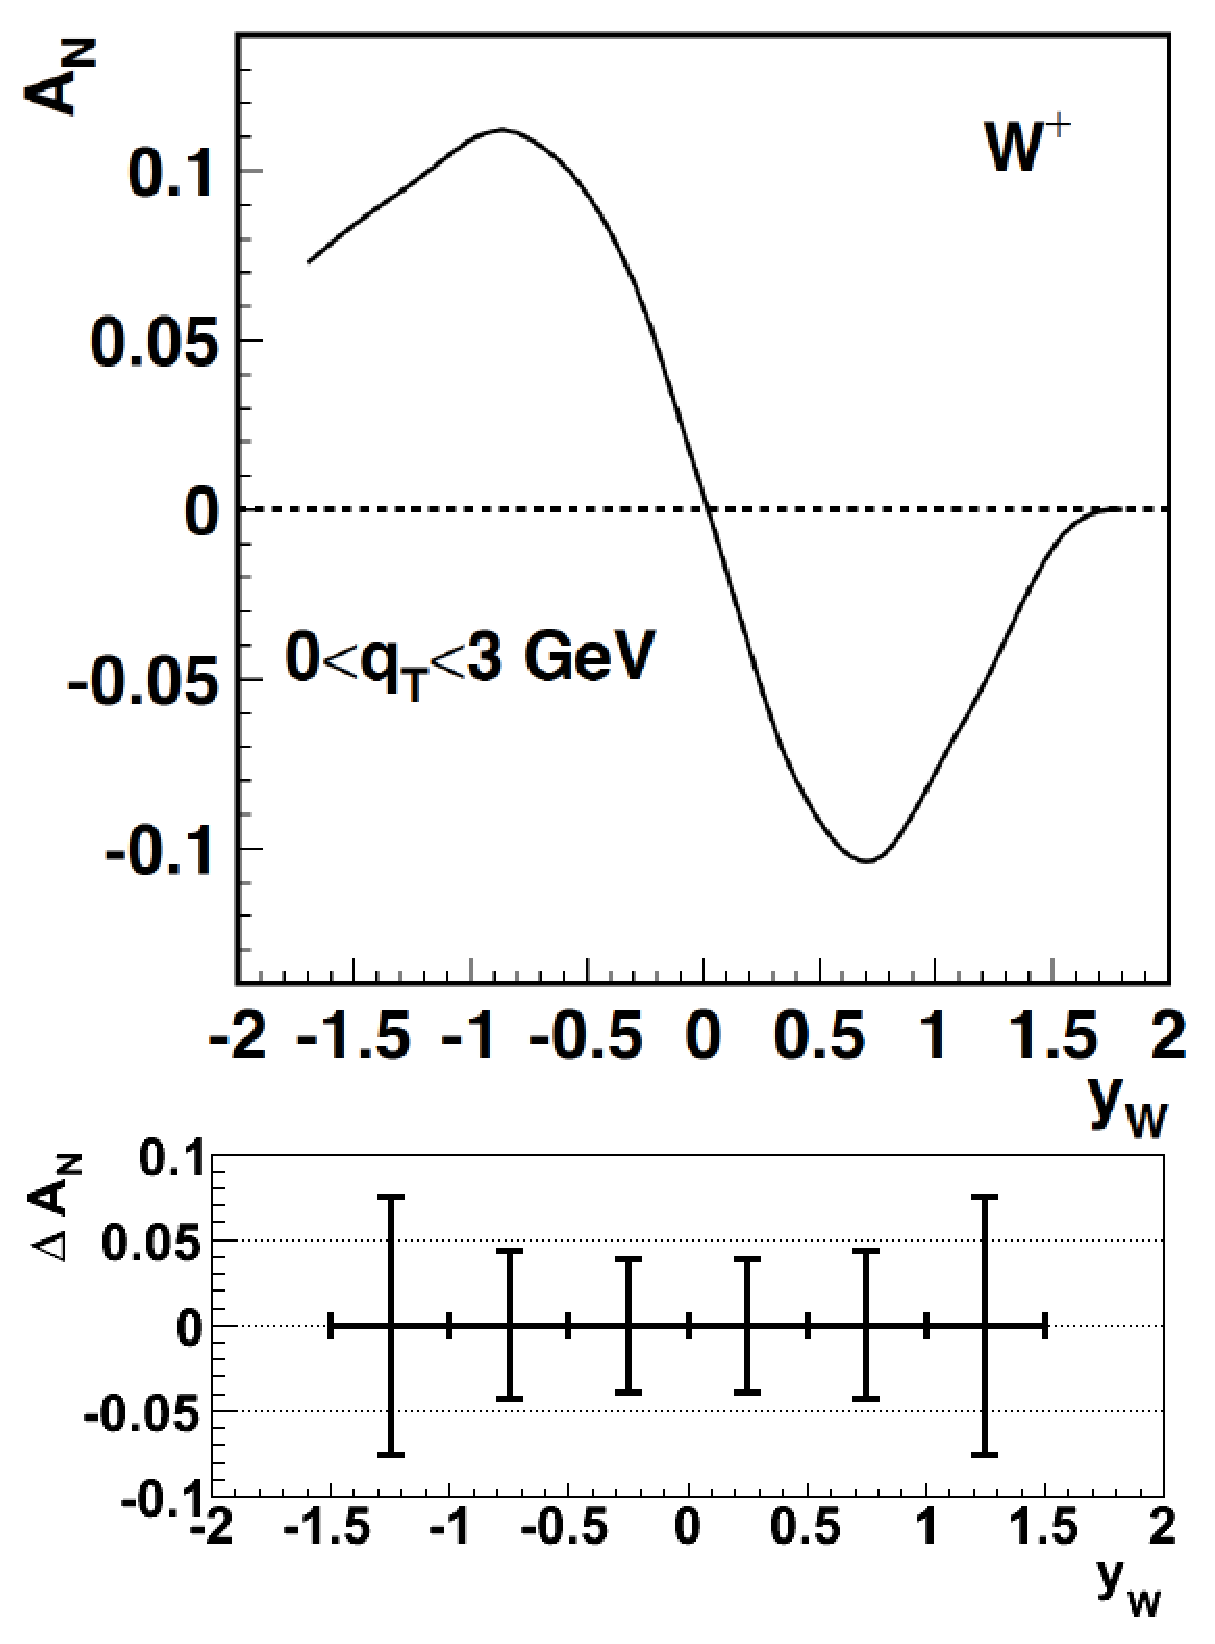
\includegraphics[width=0.49\textwidth]{images/anapow_w_plus} \label{fig:MC_Wmeas_stat_plus} }
\subfloat[$W^-$]{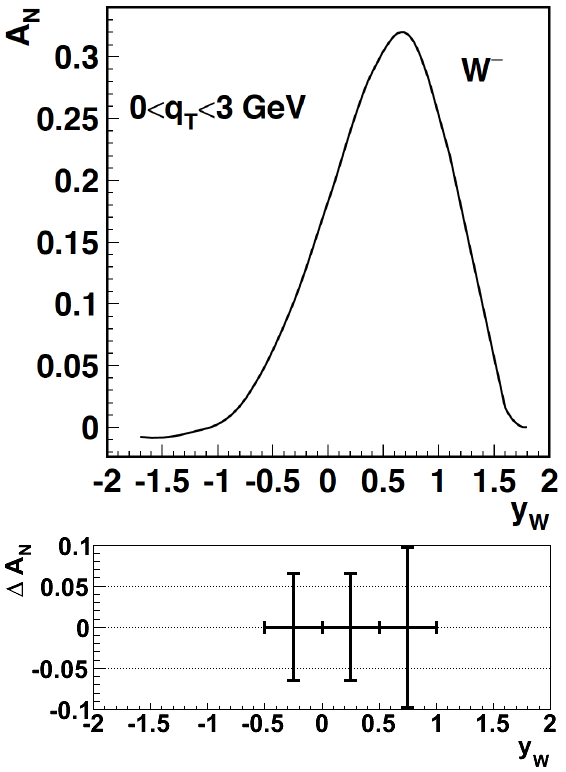
\includegraphics[width=0.49\textwidth]{images/anapow_w_minus}\label{fig:MC_Wmeas_stat_minus}}

\caption[]{Expected statistical uncertainties for measured asymmetry $A_N$ of
$W^+$ \subref{fig:MC_Wmeas_stat_plus} and $W^-$ \subref{fig:MC_Wmeas_stat_minus}
decaying leptonically at STAR as a function of the boson's rapidity.}

\label{fig:MC_Wmeas_stat} 
\end{figure}

%}}}


\section{Asymmetry measurement}
%{{{

For the SSA measurements we are interested in the proton interactions
$p^{\uparrow/\downarrow} p \to W^\pm \to e^\pm \nu_e$ in which the spin direction of one
of the protons is irrelevant, \textit{i.e} unpolarized protons. In the
experiment we can separately measure full and differential cross sections for
spin-up ($\sigma_\uparrow$), spin-down ($\sigma_\downarrow$), and unpolarized
($\sigma_0$) interactions which are related as:

\begin{align}
\sigma_\uparrow   &= \sigma_0 (1 + A_N ), \\
\sigma_\downarrow &= \sigma_0 (1 - A_N ).
\end{align}

In the following we assume that the polarization vector does not significantly
deviate from the vertical direction given by the normal unit vector $\vec n$
along the vertical $y$ axis so, the notation is $P \equiv \vec{P} \cdot
\vec{n}$. We also assume the same magnitude of the polarization vector for
spin-up and spin-down bunches, \textit{i.e.} $P = P_\uparrow = P_\downarrow$.
For unpolarized cross section $\sigma_0 \equiv (\sigma_\uparrow +
\sigma_\downarrow)/2$ the asymmetry $A_N$ is expressed as:

\begin{align}
\label{eq_anapower}
A_N &= \frac{\sigma_\uparrow - \sigma_\downarrow}{\sigma_\uparrow +
   \sigma_\downarrow}.
\end{align}

The number of recorded events in which the particle is produced with momentum
$p_T$ at angle $\Omega$ is:

\begin{align}
\frac{dN_{\uparrow/\downarrow}}{d\Omega dp_T}(\Omega, p_T) &=
   {\cal L}_{\uparrow/\downarrow} \frac{d\sigma_0}{d\Omega dp_T}(\Omega, p_T)
   \varepsilon(\Omega, p_T) \big( 1 \pm A_N(\Omega, p_T) P \big),
\label{eq:yield_diff}
\end{align}

\noindent
where detection efficiency $\varepsilon$ does not depend on the spin direction
of the interacting proton. In fact, individual events can be tagged by the
nominal spin of colliding protons. We thus can bin all collected data  in four
bins $N_{\uparrow\uparrow}$, $N_{\uparrow\downarrow}$,
$N_{\downarrow\uparrow}$, and $N_{\downarrow\downarrow}$. For the SSA
measurement the polarization of one of the beams is ignored by combining the
yields with opposite spins, \textit{e.g.}

\begin{align}
N_{\uparrow}   \equiv N_{\uparrow0}   &= N_{\uparrow\uparrow}   + R_{\frac{0\uparrow}{0\downarrow}} N_{\uparrow\downarrow},\\
N_{\downarrow} \equiv N_{\downarrow0} &= N_{\downarrow\uparrow} + R_{\frac{0\uparrow}{0\downarrow}} N_{\downarrow\downarrow},
\end{align}

\noindent
where re-weighting factor $R_{\frac{0\uparrow}{0\downarrow}}$ addresses a
possible relative difference in the spin-up and spin-down intensities of the
other beam. Studies have shown that $R_{\frac{0\uparrow}{0\downarrow}} \approx
1$ with good precision.

We bin our data sample in three observable variables $\{y, \phi, p_T\}$ with
center and width of the $i$-th bin being $\{y_i, \phi_i, p_{T,i}\}$ and
$\{\Delta y_i, \Delta\phi_i, \Delta p_{T,i}\} \equiv \{\Delta\Omega_i\{y_i,
\Delta\phi_i\}, \Delta p_{T,i}\} \equiv \Delta_i$ respectively. The number of
events in each bin, $N_i$, is calculated by integrating both sides
of~\eqref{eq:yield_diff} within the bin:

\begin{align}
N_{\uparrow/\downarrow, i} =
   \int\limits_{\Delta_i} \frac{dN_{\uparrow/\downarrow}}{d\Omega dp_T} d\Omega dp_T.
\end{align}

\noindent
In that bin we assume the average value:

\begin{align}
A_{N,i} = \frac{1}{\Delta_i} \int\limits_{\Delta_i} A_N d\Omega dp_T,
\end{align}

\noindent
and similarly for the cross section ($\sigma_{0,i}$) and efficiency
($\varepsilon_i$). Finally, for the yields in each bin we can write:

\begin{align}
N_{\uparrow/\downarrow, i} = {\cal L}_{\uparrow/\downarrow} \sigma_{0,i}
\varepsilon_i \Delta\Omega_i \Delta p_{T,i} \left( 1 \pm A_{N,i}(\Omega, p_T) P \right)
\label{eq:yield}
\end{align}

The spacial distributions of the physical asymmetry and the cross sections are
the same for the spin-up and spin-down interactions with respect to the spin
direction. We can use this fact to easily get rid of the  quantities of no
interest in \eqref{eq:yield}. This is achieved by constructing geometric
means $\sqrt{N_\uparrow(\phi_i)N_\downarrow(\phi_i+\pi)}$ and
$\sqrt{N_\uparrow(\phi_i+\pi)N_\downarrow(\phi_i)}$ of the yields


\begin{align}
N_\uparrow(\phi_i)       &= {\cal L_\uparrow}
   \sigma_{0}(\phi_i) \varepsilon(\phi_i)    \Delta\Omega_i \Delta p_T \left( 1 + A_{N}(\phi_i) P \right) \\
%
N_\uparrow(\phi_i+\pi)       &= {\cal L_\uparrow}
   \sigma_{0}(\phi_i+\pi) \varepsilon(\phi_i+\pi)    \Delta\Omega_i \Delta p_T \left( 1 + A_{N}(\phi_i+\pi) P \right)
\end{align}


\begin{align}
N_\downarrow(\phi_i+\pi) &= {\cal L_\downarrow}
   \sigma_{0}(\phi_i+\pi) \varepsilon(\phi_i+\pi) \Delta\Omega_i \Delta p_T \left( 1 - A_{N}(\phi_i+\pi) P \right) \\
%
N_\downarrow(\phi_i) &= {\cal L_\downarrow}
   \sigma_{0}(\phi_i) \varepsilon(\phi_i) \Delta\Omega_i \Delta p_T \left( 1 - A_{N}(\phi_i) P \right)
\end{align}


Using the relations for the asymmetry and cross section $A_{N}(\phi_i+\pi) =
-A_{N}(\phi_i)$, $\sigma_0(\phi_i+\pi) = \sigma_0(\phi_i)$ we get for $A_N$


\begin{align}
A_{N, i} = \frac{1}{P} \frac{%
\sqrt{N_{\uparrow}(\phi_i)N_{\downarrow}(\phi_i+\pi)} -
\sqrt{N_{\uparrow}(\phi_i+\pi)N_{\downarrow}(\phi_i)}
}}}
\newpage

\begin{thebibliography}{9}

\bibitem{WCrossSecRun9}
``Measurement of the W and Z Production Cross Sections at Mid-rapidity in Proton-Proton Collisions at $\sqrt{s} = 500$~GeV in Run~9,'' STAR~Note~0546.

%\cite{Kang:2009bp}
\bibitem{Kang:2009bp} 
  Z.~-B.~Kang and J.~-W.~Qiu,
  ``Testing the Time-Reversal Modified Universality of the Sivers Function,''
  Phys.\ Rev.\ Lett.\  {\bf 103}, 172001 (2009)
  [arXiv:0903.3629 [hep-ph]].
  %%CITATION = ARXIV:0903.3629;%%

\end{thebibliography}

\end{document}
